\section{问题一}
\subsection{问题重述}
编写一个程序,可以实现计算矩形波导在不同的$\dfrac{a}{b}$的情况下,前$5$个高次模出现的先后顺序。
用你的程序给出两组例子。
\subsection{理论基础}
由无源区Maxwell方程组:
\begin{equation}\label{1}
    \left\{
    \begin{aligned}
        \nabla\times\vec{H} & =\jmath\omega\varepsilon\vec{E} \\
        \nabla\times\vec{E} & =-\jmath\omega\mu\vec{H}        \\
        \nabla\cdot \vec{E} & =0                              \\
        \nabla\cdot\vec{H}  & =0
    \end{aligned}\right.
\end{equation}

可得波动方程(Helmholtz方程):
\begin{equation}\label{2}
    \left\{
    \begin{aligned}
        \nabla^2\vec{E} +k^2\vec{E} & =0 \\
        \nabla^2\vec{H} +k^2\vec{H} & =0
    \end{aligned}\right.
\end{equation}

采用纵向分量法,可以得到如下方程:
\begin{equation}\label{3}
    \dfrac{\partial }{\partial z} \to -\gamma\quad
    \left\{
    \begin{aligned}
        E_z & =E(x,y)\mathrm{e}^{-\gamma z} \\
        H_z & =H(x,y)\mathrm{e}^{-\gamma z} \\
    \end{aligned}\right.
\end{equation}

由不变性矩阵:
\begin{equation}\label{4}
    \begin{bmatrix}
        E_x \\
        E_y \\
        H_x \\
        H_y \\
    \end{bmatrix}
    =\dfrac{1}{k_c^2}\begin{bmatrix}
        -\gamma                  & 0                       & 0               & -\jmath\omega\mu \\
        0                        & -\gamma                 & \jmath\omega\mu & 0                \\
        0                        & \jmath\omega\varepsilon & -\gamma         & 0                \\
        -\jmath\omega\varepsilon & 0                       & 0               & -\gamma          \\
    \end{bmatrix}
    \begin{bmatrix}
        \dfrac{\partial E_z}{\partial x} \\[8pt]
        \dfrac{\partial H_z}{\partial y} \\[8pt]
        \dfrac{\partial E_z}{\partial x} \\[8pt]
        \dfrac{\partial H_z}{\partial y} \\[8pt]
    \end{bmatrix}
\end{equation}
可分别得到$TE$、$TM$模的表达式:

$TE_{mn}$场分布如式\ref{5}所示。
\begin{equation}\label{5}
    \left\{
    \begin{aligned}
        H_z & =H_0\cos (\dfrac{m\pi}{a}x)\cos (\dfrac{n\pi}{b}y)\mathrm{e}^{-\gamma z}                                               \\[8pt]
        E_x & =\jmath\dfrac{\omega\mu}{k_c^2}\dfrac{n\pi}{b}H_0\cos (\dfrac{m\pi}{a}x)\sin (\dfrac{n\pi}{b}y)\mathrm{e}^{-\gamma z}  \\[8pt]
        E_y & =-\jmath\dfrac{\omega\mu}{k_c^2}\dfrac{m\pi}{a}H_0\sin (\dfrac{m\pi}{a}x)\cos (\dfrac{n\pi}{b}y)\mathrm{e}^{-\gamma z} \\[8pt]
        E_z & =0                                                                                                                     \\[8pt]
        H_x & =\dfrac{\gamma}{k_c^2}\dfrac{m\pi}{a}H_0\sin (\dfrac{m\pi}{a}x)\cos (\dfrac{n\pi}{b}x)\mathrm{e}^{-\gamma z}           \\[8pt]
        H_y & =\dfrac{\gamma}{k_c^2}\dfrac{n\pi}{b}H_0\cos (\dfrac{m\pi}{a}x)\sin (\dfrac{n\pi}{b}x)\mathrm{e}^{-\gamma z}           \\[8pt]
    \end{aligned}\right.
\end{equation}
其中$k_c^2=k_x^2+k_y^2$ , $m$表示$x$ 方向变化的半周期数,$n$表示$y$方向变化的半周期数。
$TM_{mn}$场分布如式\ref{6}所示。
\begin{equation}\label{6}
    \left\{
    \begin{aligned}
        E_z & =E_0\sin (\dfrac{m\pi}{a}x)\sin (\dfrac{n\pi}{b}y)\mathrm{e}^{-\gamma z}                                                       \\[8pt]
        E_x & =-\gamma\dfrac{1}{k_c^2}\dfrac{m\pi}{a}E_0\cos (\dfrac{m\pi}{a}x)\sin (\dfrac{n\pi}{b}y)\mathrm{e}^{-\gamma z}                 \\[8pt]
        E_y & =-\gamma\dfrac{1}{k_c^2}\dfrac{n\pi}{b}E_0\sin (\dfrac{m\pi}{a}x)\cos (\dfrac{n\pi}{b}y)\mathrm{e}^{-\gamma z}                 \\[8pt]
        H_z & =0                                                                                                                             \\[8pt]
        H_x & =\jmath\dfrac{\omega\varepsilon}{k_c^2}\dfrac{n\pi}{b}E_0\sin (\dfrac{m\pi}{a}x)\cos (\dfrac{n\pi}{b}x)\mathrm{e}^{-\gamma z}  \\[8pt]
        H_y & =-\jmath\dfrac{\omega\varepsilon}{k_c^2}\dfrac{m\pi}{a}E_0\cos (\dfrac{m\pi}{a}x)\sin (\dfrac{n\pi}{b}x)\mathrm{e}^{-\gamma z} \\[8pt]
    \end{aligned}\right.
\end{equation}

当$a>b$时,$m=1,n=0$的$\lambda_c$ 最大(或者说$f_c$最低)。因为$TM$模式中$m,n$ 都不能为$0$,所以$f_c$最大的只能是$TE_{10}$模。
矩形波导中$TE_{mn}$和$TM_{mn}$是简并的,具有相同的$k_c$ 。
由$k_c=\sqrt{k_x^2+k_y^2}=\sqrt{(\dfrac{m\pi}{a})^2+(\dfrac{n\pi}{b})^2}=\dfrac{2\pi}{\lambda_c}$,可计算出截止波长:
\begin{equation}\label{7}
    \lambda_c=\dfrac{2}{\sqrt{(\dfrac{m}{a})^2+(\dfrac{n}{b})^2}}
\end{equation}
利用式\ref{7}可以计算矩形波导在不同的$\dfrac{a}{b}$的情况下,前$5$个高次模出现的先后顺序。
亦可采用图解法,此处给出$TE.TM_{11},TE.TM_{21},TE.TM_{31},TE_{01},TE_{02},TE_{10},
    TE_{20},$\\$TE_{30},TE_{40}$的示意图。
    由式\ref{7}可推得:
    \begin{equation}\label{8}
        \lambda_c^2<\dfrac{4}{\sqrt{(\dfrac{m}{a})^2+(\dfrac{n}{b})^2}}
    \end{equation}
    令$x=\dfrac{\lambda}{a}$,$y=\dfrac{\lambda}{b}$ ,$y=\dfrac{\lambda}{b}=\dfrac{\lambda}{a}\dfrac{a}{b}=\dfrac{a}{b}x$
    可得轨迹:
    \begin{equation}\label{9}
        m^2x^2+n^2y^2<4
    \end{equation}

    现列表如表\ref{table-1}所示。
    \begin{table}[htbp]
        \centering
        \renewcommand\arraystretch{1.5}
        \caption{图解法}
        \label{table-1}
        \vspace{1em}
        \begin{tabular}{C{3cm}C{3cm}C{3cm}}
            \hline
            $TE_{10}$    & $m=1,n=0$ & $x<2$           \\
            \hline
            $TE_{01}$    & $m=0,n=1$ & $y<2$           \\
            \hline
            $TE_{20}$    & $m=2,n=0$ & $x<1$           \\
            \hline
            $TE_{02}$    & $m=0,n=2$ & $y<1$           \\
            \hline
            $TE_{30}$    & $m=3,n=0$ & $x<\frac{2}{3}$ \\
            \hline
            $TE_{40}$    & $m=4,n=0$ & $x<\frac{1}{2}$ \\
            \hline
            $TE.TM_{11}$ & $m=1,n=1$ & $x^2+y^2<4$     \\
            \hline
            $TE.TM_{21}$ & $m=2,n=1$ & $4x^2+y^2<4$    \\
            \hline
            $TE.TM_{31}$ & $m=3,n=1$ & $9x^2+y^2<4$    \\
            \hline
        \end{tabular}
    \end{table}
    \subsection{具体实现}
    编程语言:Python

    编程环境:Anaconda + VS Code + PyCharm

    依赖库:numpy、matplotlib

    程序流程图如图\ref{pic1-1}所示:
    \begin{figure}[htbp]
        \centering
        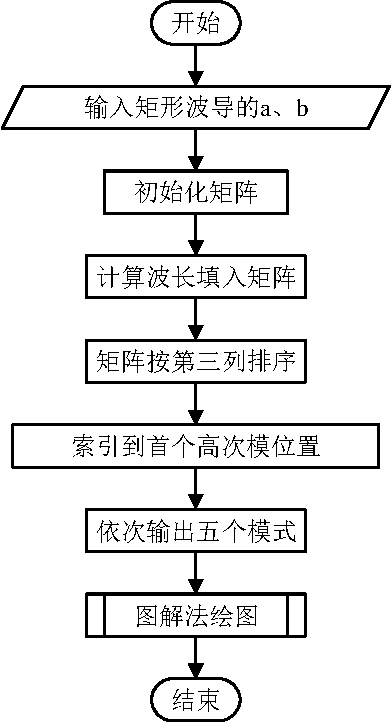
\includegraphics[width=0.4\linewidth]{figure/流程图-crop.pdf}
        \caption{程序流程图}
        \label{pic1-1}
    \end{figure}
    对初始化矩阵加以解释:第一列为矩形波导工作的模式,
$1$表示$TE$、$2$表示$TM$、$3$表示$TE$、$TM$;第二列为$m$;第三列为$n$;
    最后一列为波长,初始化为浮点数$0.0$,计算后填入正确的值。

    全部源代码见附录A。\ref{Microwave.py}
    \subsection{两组例子}
    \subsubsection{BJ-100}
    以$BJ-100$波导为例:$a=22.86\mathrm{mm},b=10.16\mathrm{mm}$ ,由以上程序可得:
    出现的前$5$个高次模为:$TE_{20},TE_{10}, TE.TM_{11},TE_{30},TE.TM_{21}$。
    \begin{figure}[htbp]
        \centering
        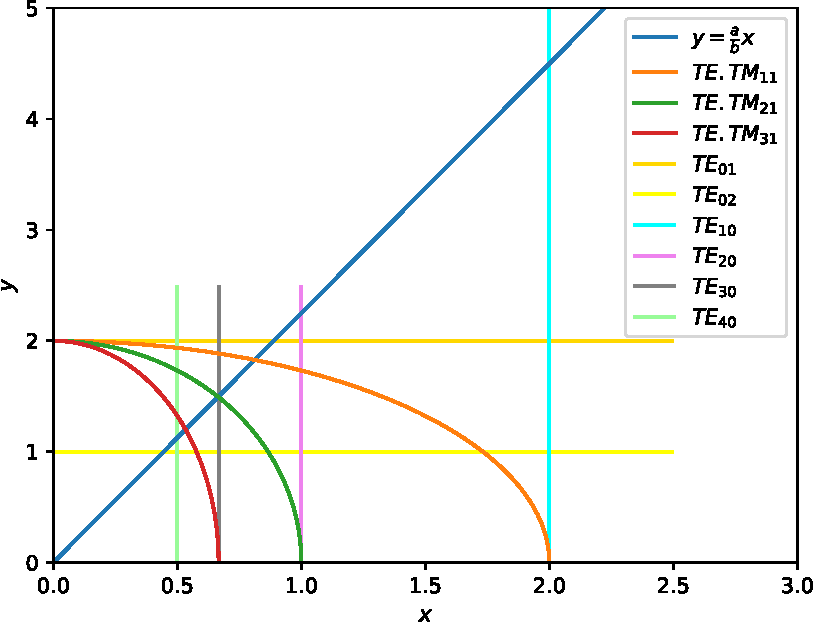
\includegraphics[width=0.7\linewidth]{figure/Microwave-BJ100-crop.pdf}
        \caption{程序流程图}
        \label{pic1-2}
    \end{figure}
    \subsubsection{BJ-120}
    以$BJ-120$波导为例:$a=19.05\mathrm{mm},b=9.525\mathrm{mm}$  ,由以上程序可得:
    出现的前$5$个高次模为:$TE_{10},TE_{20},TE.TM_{11},TE.TM_{21},TE_{30}$.
\begin{figure}[htbp]
    \centering
    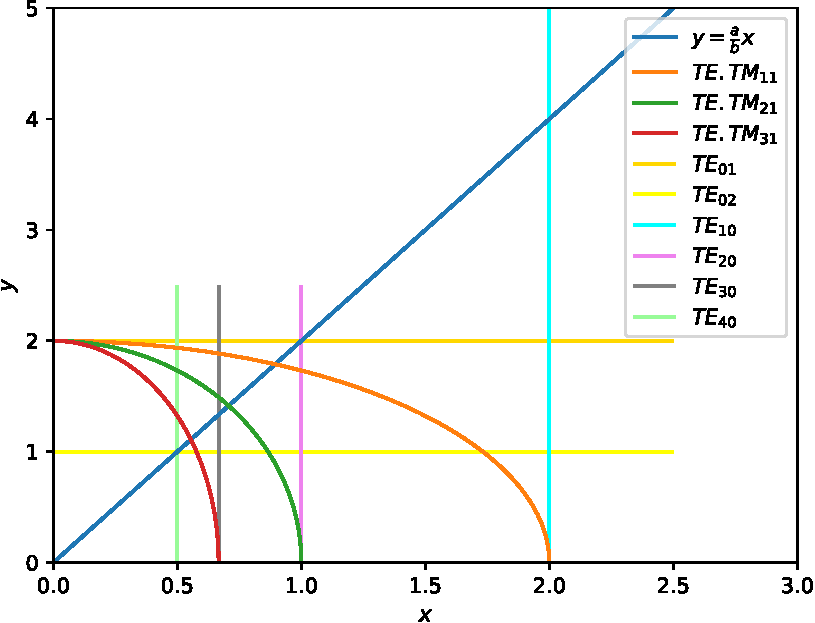
\includegraphics[width=0.7\linewidth]{figure/Microwave-BJ120-crop.pdf}
    \caption{程序流程图}
    \label{pic1-3}
\end{figure}